%===============================================================================
% $Id: ifacconf.tex 19 2011-10-27 09:32:13Z jpuente $  
% Template for IFAC meeting papers
% Copyright (c) 2007-2008 International Federation of Automatic Control
%==============================1=================================================
\documentclass{ifacconf}
\usepackage[utf8]{inputenc}
%\usepackage[english]{babel}

\usepackage{graphicx}      % include this line if your document contains figures
\usepackage{natbib}        % required for bibliography
\setcitestyle{numbers}
\usepackage{url}
\usepackage{amsmath}
\usepackage{algorithm}
\usepackage[noend]{algpseudocode}
\makeatletter
\def\BState{\State\hskip-\ALG@thistlm}

\algnewcommand\algorithmicforeach{\textbf{foreach}}
\algdef{S}[FOR]{ForEach}[1]{\algorithmicforeach\ #1\ :}

\makeatother

\pagestyle{plain}
%===============================================================================
\begin{document}
\begin{frontmatter}

\title{Autonomous Exploration Agent} 

\author{Federico Bottoni (806944)}
\author{Nassim Habbash (808292)}

\address{Complex Systems and Artificial Intelligence courses project\\for the MSc in CS at University of Milano-Bicocca \\ 
(e-mails: f.bottoni1@campus.unimib.it,\\
n.habbash@campus.unimib.it).}

\begin{abstract}
The following project proposes and evaluates an agent that attempts to minimize collisions during the search for a target in obstacle-ridden, randomly generated chaotic environments. The proposed architecture applies deep reinforcement learning, namely Proximal Policy Optimization to train the agent in the environment. Different experiments are carried out to compare the model's training and behaviour to environmental and agent's variations, underlining how classical performance measures are not always coupled with environmental performance of the agent.
\end{abstract}

\begin{keyword}
deep reinforcement learning, artificial intelligence, agent systems, environment, simulation
\end{keyword}
\end{frontmatter}
%===============================================================================

\section{Introduction}
The world is every day more automatic and controlled by machines, starting from robots like drones and rovers, through the industry 4.0 and smart-city systems, to self-driving cars and home automation. \emph{Artificial intelligence} is the common keyword of all these fields. Data-driven techniques like machine learning and reinforcement learning are useful to create predictive models capable of taking decision autonomously, specializing inferred data in the each context. 

The project consists in evaluating the ability of a reinforcement learning approach to control an agent exploring capabilities in an environment, avoiding obstacles and finding a target. The goal consists in the comparison in model behavior in variations of the system architecture - such as variations in the environment and agent models.
\citep{paper}

\section{Agent and Environment}
The agent is modeled after a simplified rover robot with omnidirectional wheels, capable of moving on the ground in all directions. The location of the agent is described by its $(x, y, \vartheta)$,
where $(x, y)$ denote a cartesian position and $\vartheta$ denotes an orientation. The agent has also a physical volume that, when there is an intersection between the collision boxes, may hit both the obstacles in the space and the goal during its movement.\\
The environment simulation is a ground with obstacles at the borders, where the agent can move on. A set of gray cubes with a bigger size than the agent are randomly generated on this plane as obstacles. The target is positioned randomly between this set of obstacles, and does present a different coloration. The agent has to find the target and reach it to consider the episode and task completed.\\
The agent can observe the space, detecting obstacles and the target through a set of LIDARs that create a array of surveying rays: these are time-of-flight sensors which provide information about the distance between the agent and the observed entity for each ray. If a ray is not long enough to reach an object because it is too far away, the data provides the over-maximum-range information to the agent.\\
The possible actions that the agent can perform are:
\begin{itemize}
    \item Move forward or backward
    \item Move to the left or to the right
    \item Rotate counterclockwise or clockwise (yaw rotation)
\end{itemize}
The agent can also combine the actions, for example going forward-right while rotating counterclockwise.\\\\

The environment is generated for each episode, and as such, no two identical episodes are played by the agent. That being said, the disposition of the elements in the environment (obstacles, target and agent) is static, as, with the exception of the agent, the elements are fixed in place after being generated.\\
The possible interactions are between the agent with an obstacle and the agent with the target. A collision happens when there is an intersection between the bounding boxes of two entities: if the collision happens between agent and obstacles, the agent suffers a penalty, if the collision happens between agent and target, the episode ends successfully, as the agent achieved the goal. 

\begin{figure}[!hb]
\begin{center}
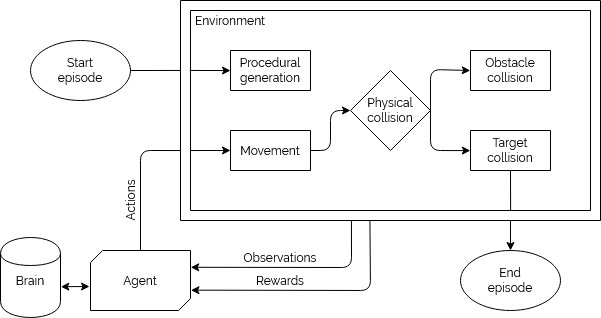
\includegraphics[width=\linewidth]{res/agent.png} 
\caption{Schematized system architecture} 
\label{fig:agent_model}
\end{center}
\end{figure}

\subsection{Approach} 
A great technique which can be adopted in order to solve agent-environment simulation tasks is \emph{Reinforcement Learning}. In the past couple of years there have been many successful and remarkable applications in the robot and locomotive field, such as \citep{heess2017emergence} and \citep{wenhao2018}. This approach provides many benefits: it is possible to conduct safe experimentation in a (safe), simulated environment, which with current technology allows for a good approximation of reality.  It also allows the models to go through millions of iterations to learn the optimal behaviour, and in some fields - such as robot movement - the RL approach currently outperforms classic heuristic and evolutionary methods \citep{suttonbarto}.
As such, the choice to use RL for this task is motivate both by the literature and the task's domain. \\
Generally, a Reinforcement Learning system is comprised of the following components:
\begin{enumerate}
    \item A policy function, which is a mapping between the state space (observations) and the action space of the agent
    \item A reward signal, which defines the goal of the problem, and is sent by the environment to the agent at each time-step
    \item A value function, which defines the expected future reward the agent can gain from the current and all subsequent future states
    \item A model, which defines the actual behaviour of the environment
\end{enumerate}
Different RL algorithms may implement all or some of these components, bringing different flavors to the learning capabilities of the system.
\emph{Policy Gradient} methods are a type of Reinforcement Learning techniques that rely upon optimizing parametric policies toward a progressive convergence by gradient descent. The method utilized to identify the expected agent's policy in this setting is \emph{PPO} (Proximal Policy Optimization) which is a policy gradient method which also shares some of the benefits of \emph{TRPO} (Trust Region Policy Optimization) \citep{ppo}.\\
The trade-off between \emph{exploration} and \emph{exploitation} takes an important spotlight in the implementaton of RL algorithms. Here is necessary to look for the correct balance of these two learning approaches to avoid the development of a kind of "shy" behavior (case of no exploration) or a kind of "reckless" one (case of no exploitation). To find the right balance a curiosity reward was added to the extrinsic one in order to relate the final reward signal to both exploration of the state-space and the exploitation of the knowledge for the task.

\section{System architecture}
The simulation has been developed using Unity3D as the main platform.
Unity is a game development platform consisting of a game engine and an IDE. Unity offers a rich visual editor to create 3D or 2D environments, a solid physics engine, and C\# scripting capabilities.
The simulation software has been built as Unity3D application using the APIs provided by "The Unity Machine Learning Agents Toolkit", \emph{ml-agents} (with \emph{Tensorflow} as backend).

\subsection{Frameworks} 
Unity3D is a well-established open-source game engine. It provides a lot of out-of-the-box functionalities including tools to assemble a scene, the 3D engine to render it, a physics engine to make the objects react in a realistic way, tons of plugins applicable to components and many others. The engine allows to create components that can be physically in the scene or just virtual and attach a C\# script to them. For each component is possible to handle individually the different parts of it: in our case the object as component (Unity's GameObject), its physics (if it's declared as RigidBody) and its role in the learning system (Agent, Academy and others). The component's life begins with a initialization and then an infinite refresh of the state, the engine provides the handler methods of these phases customizing them through an event-driven programming. \\
Unity3D's engine way of keeping track of time and events is stratified on a pipeline: physics, game logic and scene rendering are each computated sequentially, async and at different frequency. That makes it so that physics updates, which consist in movement of objects or collision physics, happen at a different rate than logic happening in normal updates. This, in a game development scenario is sometimes treated by buffering inputs or other techniques, while in a simulation environment, such as this, does pose a slight inconvenience in the case of really precise simulations.\\
\textbf{Ml-Agents} is an open-source Unity3D plugin that enables games and simulations to serve as environments for training intelligent agents. It also provides implementations (based on TensorFlow) of state-of-the-art algorithms, including PPO and a a curiosity module for the agent's reward.

\subsection{System design} 
Learning is possible thanks to a few extendable components that implement the parts of the system: the \textbf{Agent}, which has a module of the same name, is the protagonist of the scene: it can observe the environment declaring the observation tool; it can perform significant actions in the the system customizing the motion of the physical body in the environment, overriding the \emph{AgentAction} method; it can calculate the cumulative reward in a custom function and declare the success of an episode if the target is hit and declare the failure if the the cumulative reward reach the minimum value -5.\\
The \textbf{Environment} is composed of different modules: the first is the \emph{Academy} class, which is a hub routing information - whether it's observations from the environment or inferences made by the models - in and out of the system. The second one is the environment in its physical part: it is represented in the \emph{TrainingArea} class and is made up by the area, the obstacles, the target. This module handles the spawn of the obstacles, the target and the agent in the environment according to the specified environmental parameters injected by the Academy. It has also a role in the composition of the information present above the scene, which are the number of collisions and the the actual cumulative reward. Visually the environment consists in a little light blue cube (agent) on a grey plane with borders with some sparse white and gray cubes (obstacles) and one of them is orange (target). \\ 
The \textbf{learning} happens in the \emph{Brain}: this module is connected to another one that contains an implementation of the PPO algorithm. Once the training phase ends, the ML-Agents framework generates a model file which can be connected to the brain and used directly for inference: it gets the observations of the agent, during the simulation phase, and generate the best action to maximize the reward signal.

\begin{figure}[H]
\begin{center}
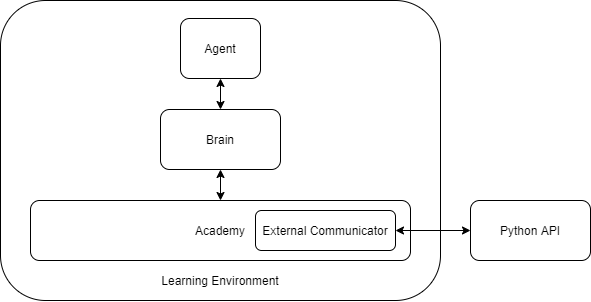
\includegraphics[width=\linewidth]{res/learning_env.png} 
\caption{Learning according to the ml-agents framework: the brain communicate to the Tensorflow module through the external communicator of the Academy} 
\label{fig:learning_env}
\end{center}
\end{figure}


\begin{figure}[H]
\begin{center}
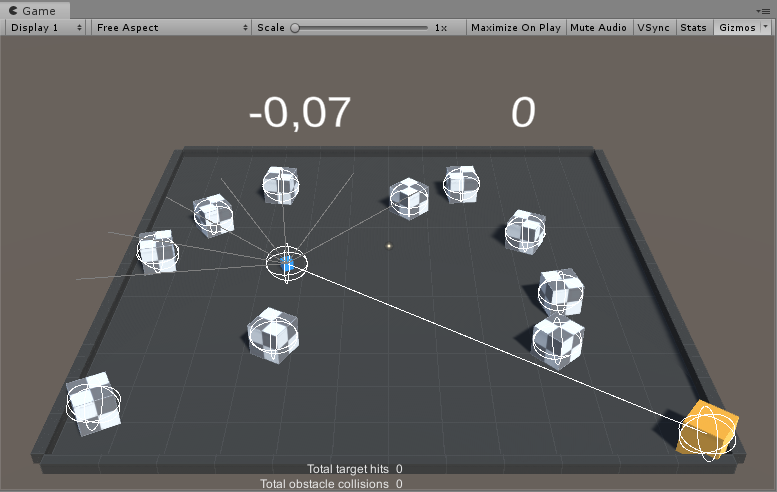
\includegraphics[width=\linewidth]{res/un_env.png} 
\caption{Environment: the blue cube is the agent, the checkerboard pattern cubes are the obstacles and the orange cube is the target. The environment is generated considering the distance between agent and target (white line connecting both) and the minimum spawn distance (the white sphere around objects) to ensure a parametrized distribution between objects in the scene. The agent collects observations through its LIDAR array (white rays exiting the agent).} 
\label{fig:graphical_env}
\end{center}
\end{figure}

The environment is rendered in the beginning of each episode with the described procedure "SpawnObjects".

\begin{algorithm}
\caption{Spawn of the environment objects}\label{alg:spawn}
\begin{algorithmic}[1]
\Procedure{SpawnObjects}{minDistance, minAT}
\State $\text{occupiedPositions} \gets \textit{EmptyList}$
\State $\text{sceneObjects} \gets \text{agent} \cup \text{target} \cup \text{obstacles}$
\ForEach {$\text{sceneObject} \in \textit{sceneObjects} $}
\State $\text{foundLocation} \gets \text{FALSE}$
\Repeat
\If {$\text{sceneObject is } \textit{target}$}
\State {$\text{relPos} \gets$ Vector2(minAT, randAngle)}
\Else
\State {$\text{relPos} \gets$ Vector2(randX, randY)}
\EndIf
\State{$\text{position} \gets \text{clampVect(relPos, areaBounds)}$}
\State{$\text{distanceAT} \gets \left\| \text{agent.position - position} \right\|$}
\State \begin{varwidth}{\linewidth}
      \textit{checkedSpawn}~$\gets$~checkPosition(\par
        \hskip\algorithmicindent\hskip\algorithmicindent\hskip\algorithmicindent position,\par
        \hskip\algorithmicindent\hskip\algorithmicindent\hskip\algorithmicindent sceneObject.colliderRadious,\par
        \hskip\algorithmicindent\hskip\algorithmicindent\hskip\algorithmicindent occupiedPositions,\par
        \hskip\algorithmicindent\hskip\algorithmicindent\hskip\algorithmicindent minDistance);
      \end{varwidth}
\State{$foundLocation \gets distanceAT - minAT \textless \text{tolerance} \And \text{checkedSpawn}$}
\State{$\text{attempts} = \textit{attempts} - 1$}
\Until{$! \text{foundLocation} \And \text{attempts} > 0$}
\State{$\text{sceneObject}\text{.position} = \text{position}$}
\State{$\text{sceneObject}\text{.orientation} = \text{randomAngle()}$}
\State{occupiedPositions.add(sceneObject)}
\EndFor
\EndProcedure
\end{algorithmic}
\end{algorithm}

Given the obstacles, the agent, the target and given the dynamic parameters \emph{minAT} ("Target Distance" is the distance, with an uncertainty of 5 units, between the agent and the target at spawn time) and \emph{minDistance} ("Min Spawn Distance" is the minimum distance between each element of the environment), the script computes the position and orientation of each element of the scene, ensuring the uniform distribution of the objects in the environment and the distance between the agent and target according to the parameters.

\begin{table}[ht]
\centering
\caption{Static environmental parameters}
\begin{tabular}[t]{cc}
\hline
\textbf{Agent parameters}&\\
\hline
Dimensions&1x1x1\\
Max linear velocity&5\\
Max angular velocity&$\frac{5}{3} \pi$\\[0.1cm]
\hline
\textbf{Sensor parameters}&\\
\hline
N.LIDARS&14\\
Maximum range&20\\
Field of view&[-$\frac{2}{3} \pi$; $\frac{2}{3} \pi$]\\[0.1cm]
\hline
\textbf{Environment parameters}&\\
\hline
Level area&50x50\\
Target dimensions&8x8x8\\
Obstacle dimensions&8x8x8\\
\end{tabular}
\end{table}%

\section{3D Maneuvering System} % agente, env, osservazioni, azioni, training, problemi
The system also has a 3D Maneuvering System, which extends the 2D model by adding the \emph{up-down} translations and the rotation \emph{pitch} to the agent. \emph{Roll} was not implemented because it would not provide a big change of perspective to the agent's observation that, in relation to the increasing of complexity of the problem, was not necessary. The agent is able to observe the environment using a bigger set of LIDARS that consists in 5 groups of rays placed in order to gather information from different vertical positions.

\begin{table}[ht]
\centering
\caption{Parameters of the levels of LIDARS}
\begin{tabular}[t]{cc}
\textbf{3D Sensor parameters}&\\
\hline
N.LIDARS&42\\
Maximum range&40\\
Horizontal Field of View &[-$\frac{2}{3} \pi$; $\frac{2}{3} \pi$]\\[0.1cm]
Vertical Field of View &[-$\frac{1}{4} \pi$; $\frac{1}{4} \pi$]\\[0.1cm]
\hline
\end{tabular}
\end{table}%

This different environment consists in a transparent empty cube where the obstacles, the target and the agent are spawned according to the 3D version of the same algorithm "SpawnObjects3D", at the beginning of the episode but considering the entire 3D pose (6 degree-of-freedom of position and orientation). In this separate environment the agent is able to move in the static space and to look for the target in all the directions.\\

\begin{figure}[H]
\begin{center}
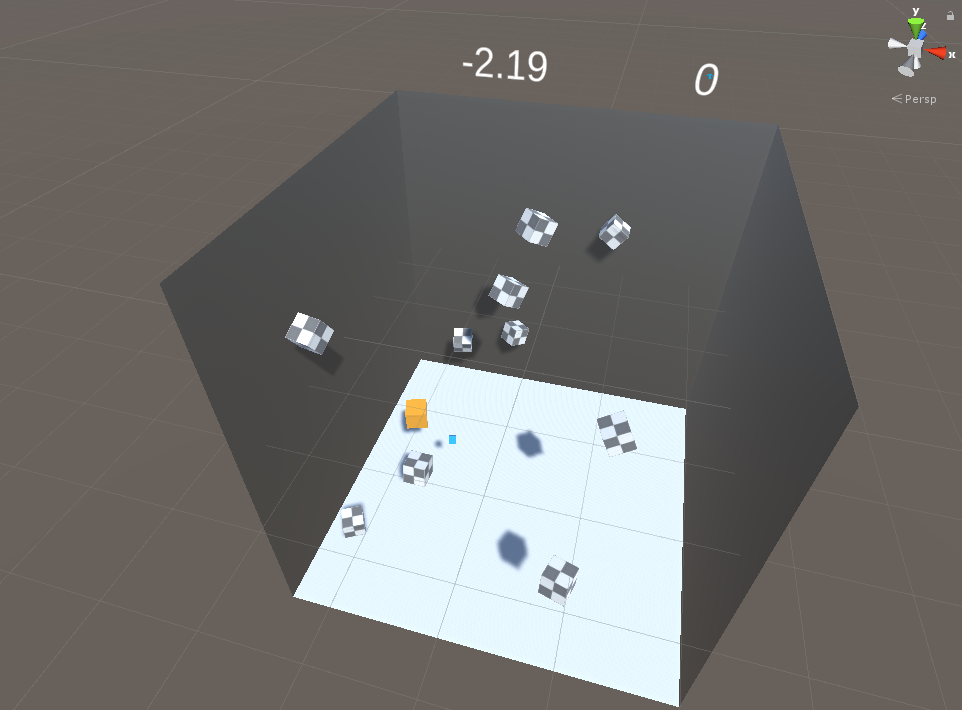
\includegraphics[width=\linewidth]{res/un_3denv.png} 
\caption{3D maneuvering environment} 
\label{fig:graphical_env}
\end{center}
\end{figure}

\section{Learning System} %Il rinforzo dellintelligenza, processo di training,
The project presents a solution using Proximal Policy Optimization. PPO is a state-of-the-art algorithm released by OpenAI \citep{ppo}. This method belongs to the policy-gradients family of RL approaches, which consist of on-policy approximation of the policy function itself. The function is approximated through a neural network, in order to produce the policy giving the maximum cumulative reward.

\subsection{Reward signal} % inizializzazione, hit target, penality, time, external, curiosity
The reward signal is composed of:
\begin{itemize}
    \item Extrinsic: the canonical one which depends on the correctness of the agent's choices
    \item Intrinsic: the \emph{curiosity} of the agent
\end{itemize}
The first one is the sum between the effective reward and the \textbf{penalty} (negative reward): when the agent hits the target, it earns a positive reward; if it hits an obstacle a penalty of $collisions*0.1$ is assigned and with the time progression an additional penalty is $time*0.001$ (values are related to the baseline case).\\
The second one is a curiosity module that consists in two networks: an inverse and a forward model. The first one takes the current and next observation of the agent, encodes them, and uses the encoding to predict the action that was taken between the observations; the second one, which takes the encoded current observation and action, predicts the next encoded observation. The difference between the predicted and actual encoded observations (loss of the forward model) is used as the intrinsic reward, so the more surprised the model is, the larger the reward will be. \citep{curiosity}

\begin{figure}[!ht]
\begin{center}
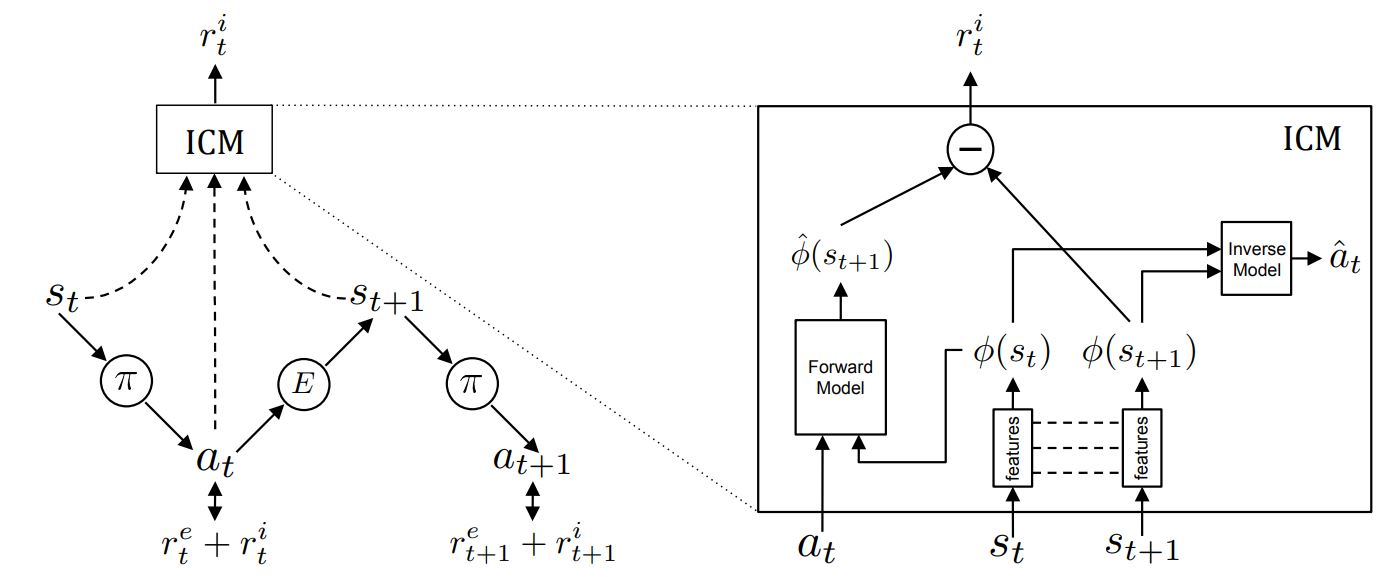
\includegraphics[width=\linewidth]{res/curiosity.JPG} 
\caption{Curiosity module as represented in \citep{curiosity}} 
\label{fig:curiosity}
\end{center}
\end{figure}

\subsection{Curriculum learning} 
The training phase of a reinforcement learning project usually is quite slow in reaching the convergence of a desired policy, especially because the algorithm is an implementation of policy gradient. Ml-Agents allows the user to enable the "curriculum" version of the learning experience in order to speed up this phase: it consists in changing the environment during the training experience in order to make the agent's task harder little by little. It's possible to distribute the training in different "difficulty levels" (lessons) and the agent can pass them getting a certain value of cumulative reward for each level. \\
The difficulty is given by some dynamic parameters which are different between the lessons:

\begin{itemize}
    \item \textbf{Reward thresholds} is expressed in decimal number and represents the agent's reward target to change lesson;
    \item \textbf{Number of obstacles} sparse inside the environment;
    \item \textbf{Min spawn distance} is the distance between each element in the scene;
    \item \textbf{Target distance} from the agent at the spawn time, with uncertainty of 5 units;
    \item \textbf{Penalty offset} is and additive value to the canonical penalty function.
\end{itemize}

\subsection{Parallel learning}
The framework allows for training multiple agents sharing the same brain - thus parallelizing the environment-agent interactions. The system was built as a prefab and it was replicated in order to speed up the training phase: it was cloned 25 times and, according to some tests, the time needed to build a similar policies decreased of 25 times.

\begin{figure}[!hb]
\begin{center}
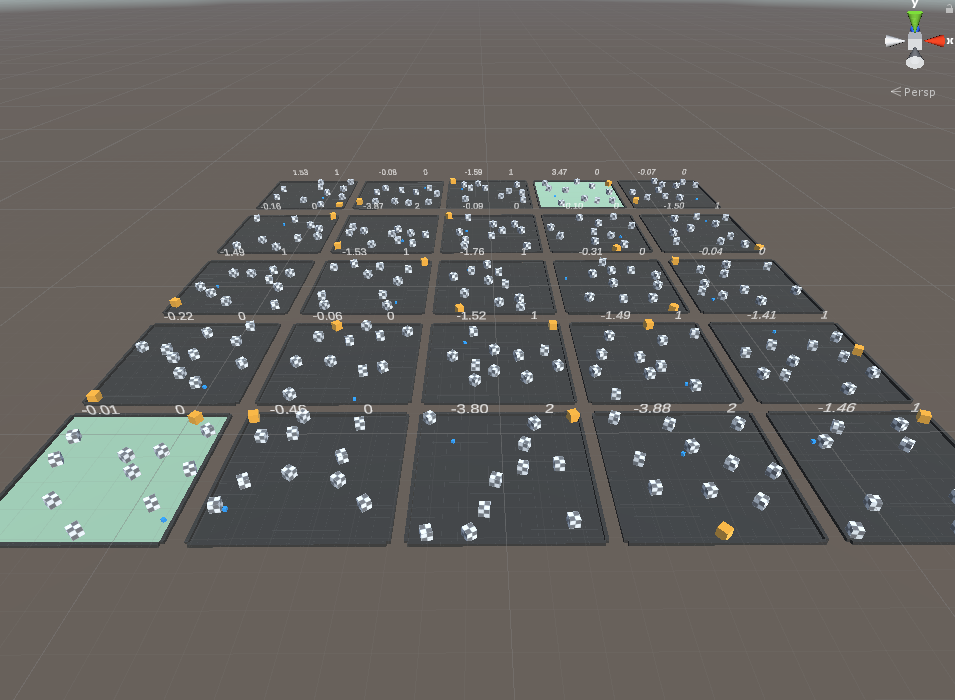
\includegraphics[width=\linewidth]{res/un_parenv.png} 
\caption{Parallel training session with 25 instances training on the same brain/model} 
\label{fig:graphical_env}
\end{center}
\end{figure}

\section{Experiments}
Different scenarios for the analysis of the effectiveness of the proposed system have been investigated. All the models shared the same hyperparameters, that are reported as following:

\begin{table}[ht]
\centering
\caption{Models hyperparameters, shared by all experiments}
\begin{tabular}[t]{cc}
\hline
\textbf{Hyperparameters}&\\
\hline
Batch size&512\\
Buffer size&4096\\
Number of layers&3\\
Hidden units&256\\
Number of epochs&6\\
Learning rate&6.0e-4\\
Epsilon&0.14\\
Beta&5.0e-3\\
Lambda&0.95\\
Max steps&1.0e7\\
\hline
\textbf{Extrinsic reward signal}&\\
\hline
Strength&1\\
Gamma&0.9\\
\hline
\textbf{Curiosity reward signal}&\\
\hline
Strength&0.02\\
Gamma&0.99\\
Encoding size&65\\
\end{tabular}
\end{table}%

The main differences between scenarios consist in:
\begin{enumerate}
    \item Curriculum environment parameters
    \item Penalty function
    \item Observation source (LIDAR or camera)
    \item 3D maneuvering environment
\end{enumerate}

Comparison between the scenarios is conducted on two aspects: one is through the comparison of the classic performance measures in a Reinforcement Learning setting, such as cumulative reward, policy and value losses, episode length, entropy and extrinsic and intrinsic rewards distribution.
The other aspect is an \textbf{environmental} performance comparison, conducted through three performance measures pertaining to the investigated setting, these being \textbf{collisions per minute} (CPM), measuring the mean number of collisions made by the agent on obstacles, \textbf{targets per minute} (TPM), measuring the mean number of goal targets successfully reached by the agent and \textbf{collisions per target} (CPT), measuring the mean number of collisions the agents does before getting to a target. As models between scenarios have been trained with varying curricula and environments, these measures estimate the performance of every model on a shared environment, making comparison between the models happen on the same plane and circumstances.

The performance has been measured in a parallel fashion: 25 agents have been let in inferencing for 5 minutes in total, accounting for 125 minutes of agent-time to measure the CPM and TPM.

All training sessions have been conducted on CPU (Intel I5-6500) and elapsed from 4 to 7.5 hours for the 2D maneuvering environments to 24 hours for the 3D maneuvering environment.
It's important to note how the variations between scenario on the chosen axes and available hardware brought a certain drawback: while every scenario ran for a discrete length of time, the number of steps taken by each experiment is not constant. In particular, experiments using the camera as an observation source managed to \textbf{reach less} than $1/6$th steps compared to the other experiments, due to the more complex pipeline involving a image encoding through a CNN.

\subsection{Baseline}
The first experiment acts as a baseline for other variations, and was conducted on the following parameters:
\begin{enumerate}
    \item Fixed parameters:
        \begin{table}[ht]
            \centering
            \begin{tabular}[t]{cc}
                Number of obstacles&10\\
                Min spawn distance&2\\
                Target distance&45\\
            \end{tabular}
            \end{table}%
        \iffalse
        \begin{enumerate}
            \item Number of obstacles: 10
            \item Min spawn distance: 2
            \item Target distance: 45
            \item LIDAR ray length: 20
        \end{enumerate}
        \fi
    \item Penalty function: $$p=collisions*0.1+time*0.001$$
    \item Observations source: LIDAR set, ray length=20
    \item 2D maneuvering environment
\end{enumerate}

The parameters in this setting generate fairly open environments with at most 10 obstacles. The minimum distance between obstacles is 2 units, while the target spawns at a distance of 45 units, which is more then half of the environment size.
\begin{table}[ht]
\centering
\caption{Baseline model environmental performances}
\label{tab:baseline}
\begin{tabular}[t]{cc}
\hline
CPM&4,984\\
TPM&3,96\\
CPT&1.25\\
\hline
\end{tabular}
\end{table}%

Table \ref{tab:baseline} shows how the model collides roughly 5 times per minute and manages to reach a target about 4 and times per minute, making roughly \textbf{1.26} obstacles per target reached.

\subsection{Curriculum}
The second experiment implemented curriculum learning into the training pipeline. The curriculum was structured in seven lessons scaling along with the cumulative reward. Following are its settings:
\begin{enumerate}
    \item Parameters:
        \begin{table}[ht]
            \centering
            \begin{tabular}[t]{cccccccc}
                Reward thresholds&1&2&2.5&2.8&3&3.5&4\\
                Number of obstacles&8&10&13&15&17&18&20\\
                Min spawn distance&6&6&4&4&3&3&2\\
                Target distance&25&28&30&33&35&37&40\\
            \end{tabular}
        \end{table}%
    \item Penalty function: $$p=collisions*0.1+time*0.001$$
    \item Observations source: LIDAR set
    \item 2D maneuvering environment
\end{enumerate}

The parameters in this setting generate an increasingly harder environment, with the target getting farther from the agent, and the obstacles getting more cluttered and closer together.

\begin{table}[ht]
\centering
\caption{Curriculum model environmental performances}
\label{tab:curric}
\begin{tabular}[t]{cc}
\hline
CPM&10,568\\
TPM&9,616\\
CPT&1.09\\
\hline
\end{tabular}
\end{table}%

Table \ref{tab:curric} shows how the model collides roughly 10.5 times per minute and manages to reach a target about 9.6 and times per minute, making roughly \textbf{1.09} obstacles per target reached. This is a significant improvement compared to the baseline, as not only the agent is able to reach the target faster, reaching 2.6 times more targets, but also with less collisions.

\subsection{Harder penalty}
The third experiment implemented curriculum learning into the training pipeline, and added a harsher penalty to the agent. The curriculum is structured as the above experiment, with the exception of the new parameter Penalty offset. Following are its settings:
\begin{enumerate}
    \item Curriculum parameters:
        \begin{table}[ht]
            \centering
            \begin{tabular}[t]{cccccccc}
                Reward thresholds&1&2&2.5&2.8&3&3.5&4\\
                Number of obstacles&8&10&13&15&17&18&20\\
                Min spawn distance&6&6&4&4&3&3&2\\
                Target distance&25&28&30&33&35&37&40\\
                Penalty offset&0.5&1.5&2&2.5&2.5&2.5&2.5\\
            \end{tabular}
        \end{table}%
    \item Harder penalty function: $$p=p_{offset}+collisions+time*0.001$$
    \item Observations source: LIDAR set
    \item 2D maneuvering environment
\end{enumerate}

As before, the parameters generate a harder environment as the cumulative reward increase, but this time the penalty function too increases in difficulty. The rationale of this experiment is that, as the agent learns how to move to reach the target, the agent should learn to not collide frequently, but instead just search in the environment for the target smoothly. Figure \ref{fig:penalty} shows how the different penalty relate to each other and the Cumulative Reward lower limit without considering time decrease (same in all penalties).

\begin{figure}[!hb]
\begin{center}
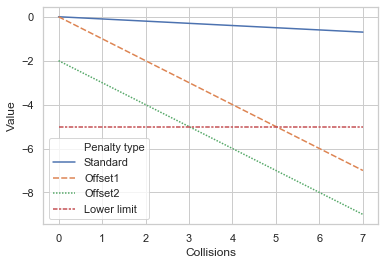
\includegraphics[width=\linewidth]{res/penalty.png} 
\caption{Penalty comparison: standard is the penalty used in most settings in the project, Offset1 and Offset2 are the penalties from the third experiment at different stages of difficulty, and the Cumulative Reward lower limit shows the number of collision before the episode aborts: Offset1 can get out with at most 5 collisions, Offset2 has a maximum of 3} 
\label{fig:penalty}
\end{center}
\end{figure}

\begin{table}[ht]
\centering
\caption{Harder penalty model environmental performances}
\label{tab:hardpen}
\begin{tabular}[t]{cc}
\hline
CPM&4,592\\
TPM&3,896\\
CPT&1.18\\
\hline
\end{tabular}
\end{table}%

Table \ref{tab:hardpen} shows how the model collides roughly 4.5 times per minute and manages to reach a target about 3.9 and times per minute, making roughly \textbf{1.18} obstacles per target reached. This model obtains results similar to the baseline, while staying below the performances the curriculum model obtained. This may be due to the harsher penalty that does not give the model time to adapt to an optimal policy.

\subsection{Camera sensors}
The fourth experiment implemented the same curriculum and penalty as the second experiment. The main difference consists in the use of a camera sensor instead of the LIDAR array, thus generating images as observations.
\begin{enumerate}
    \item Curriculum parameters: same as the second experiment
    \item Penalty function: same as the second experiment
    \item Observations source: Camera 84x84 RGB
    \item 2D maneuvering environment
\end{enumerate}

\begin{table}[ht]
\centering
\caption{Camera model environmental performances}
\label{tab:camera}
\begin{tabular}[t]{cc}
\hline
CPM&7,264\\
TPM&3,048\\
CPT&2.38\\
\hline
\end{tabular}
\end{table}%

\begin{figure}[!h]
\begin{center}
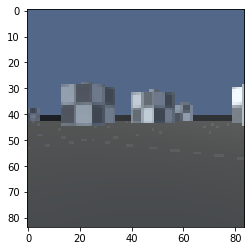
\includegraphics[width=\linewidth]{res/cameraview.png} 
\caption{Sampled observation from the agent's camera} 
\label{fig:semistr}
\end{center}
\end{figure}

The model performs significantly worse than the others. This is possibly due to the low number of steps taken by the training of the model (74k) compared to the others (700k), which did not let the algorithm converge to an optimal policy. The model manages to reach a target with roughly 2.5 obstacles hits each time, but taking roughly 3 times as much as the optimal curriculum model.

\subsection{3D maneuvering environment}
The fifth experiment implemented the same curriculum and penalty as the second experiment. The most impacting difference is the environment: instead of being 2D, thus requiring only a limited amount of movement, it is 3D, and the agent has to move in around much more space to locate and find the target.
Following are its settings:
\begin{enumerate}
    \item Curriculum parameters: same as the second experiment
    \item Penalty function: same as the second experiment
    \item Observations source: LIDAR set
    \item 3D maneuvering environment
\end{enumerate}

\begin{table}[ht]
\centering
\caption{3D maneuvering model environmental performances}
\label{tab:3d}
\begin{tabular}[t]{cc}
\hline
CPM&1.472\\
TPM&1,792\\
CPT&0.821\\
\hline
\end{tabular}
\end{table}%

The model slowly increments the cumulative reward earned as is described in Figure \ref{fig:cumrew}. After 25 hours of training, the agent manages to complete one curriculum lesson and get a positive reward value, it means that the target is reached but after a lot of research and some collisions. At the end the environment performances describes an agent which is able to find the target, with one or two collisions, but quite slowly. Probably leaving the training for other 25 hours it could converge close to the maximum reward value and learns how to find the target quickly.

\subsection{Structured environment transferability}
Taking the best performing model, the sixth experiment consisted in testing how well does the model generalize its task to structured environments - and how well does what the model learned during training in the chaotic environments transfer to other structured environments. As such, a simple fixed environment consisting of a wall with an entrance has been created, positioning the agent and the target at the two sides of the environment, and testing how the model performed. Figure \ref{fig:semistr} shows the environment.

\begin{figure}[!h]
\begin{center}
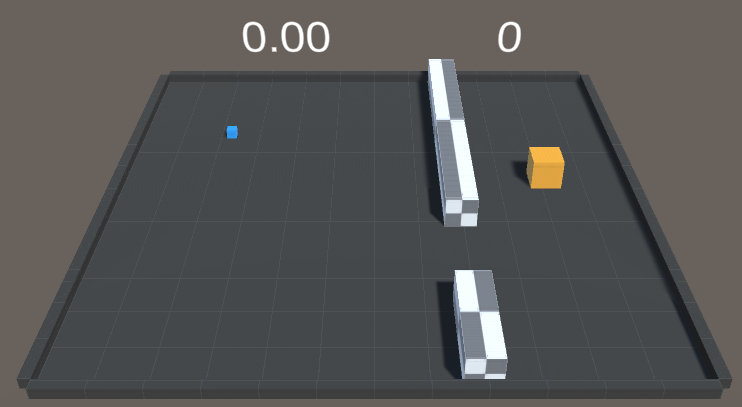
\includegraphics[width=\linewidth]{res/semistructured.png} 
\caption{Structured environment} 
\label{fig:semistr}
\end{center}
\end{figure}

\begin{table}[h]
\centering
\label{tab:curric}
\caption{Model environmental performances in the structured environment}
\begin{tabular}[t]{cc}
\hline
CPM&7,2\\
TPM&1,8\\
CPT&0.25\\
\hline
\end{tabular}
\end{table}%

The model does not perform as well as in the other environments. This seems to be due the strategy that the model has learned to be optimal for the resolution of the task at hand, seems to be \textbf{random exploration}, and will be addressed later on.

\begin{figure}[!h]
\begin{center}
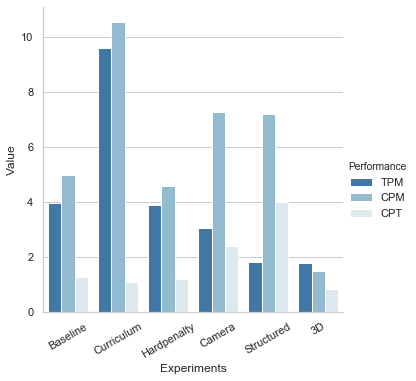
\includegraphics[width=\linewidth]{res/performances.png} 
\caption{Environmental performances comparisons between the different experiments} 
\label{fig:envperf}
\end{center}
\end{figure}

\iffalse
\begin{table}[ht]
\centering
\caption{Models behaviours}
\begin{tabular}[t]{cc}
\hline
\textbf{Model}&\textbf{Behaviour}\\
\hline
Curriculum&512\\

\end{tabular}
\end{table}%
\fi

\subsection{Classic performance measures comparison}
Following are the performance measures of the models measured during training. As the overall number of steps isn't equal between every experiments, the plot won't match for the whole length of the graph, but it does show some insight about how much it took for each training session to reach the performance reported in the previous sections.

Figure \ref{fig:cumrew} shows the cumulative reward for each experiment. The 3D maneuvering model took a long time to converge - and its lack of progress in the curriculum shows how the model still hasn't converged to an optimal policy. The other models have comparable measures: the curriculum, hardpenalty and camera models reach a similar cumulative reward - with the camera ending on top, followed by the curriculum and then hardpenalty models. This comparison shows the first caveat of the experiments: cumulative reward nonwithstanding, the curriculum model achieved way higher environmental performances than the other two models. The comparison makes even more sense if compared to the baseline model, which almost perfectly converged on a higher cumulative reward, but even then, the curriculum model achieved better performances, even with a lower cumulative reward.

Figures \ref{fig:leslen} shows, for the models employing curriculum learning, how the lessons progressed in terms of step. Here we discover a tendency for the models to reach a plateau early on in terms of steps. This may be due to the manual thresholding setup, which does not accurately increase difficulty. The only model which managed to reach the last difficulty level is the curriculum model. 

Figures \ref{fig:exrew} and \ref{fig:currew} show how the extrinsic and intrinsic rewards compare during the training lifetimes of the presented models. It is of note how the distribution of reward of the models capable to obtain a working policy shifts in time from the curiosity itself to the environmental reward, meaning a significant shift between curiosity-driven exploration and exploitation of the strategy learnt by the policy.


\begin{figure*}[!htb]
\begin{center}
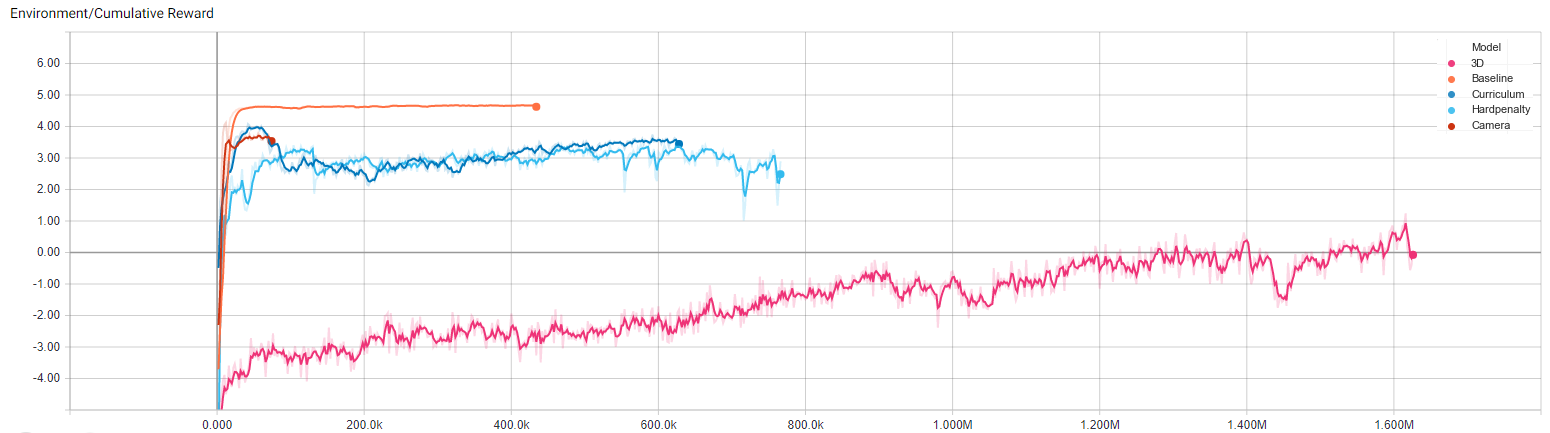
\includegraphics[width=\linewidth]{res/cumulative_reward.PNG} 
\caption{Cumulative reward} 
\label{fig:cumrew}
\end{center}
\end{figure*}

\begin{figure*}[!htb]
\begin{center}
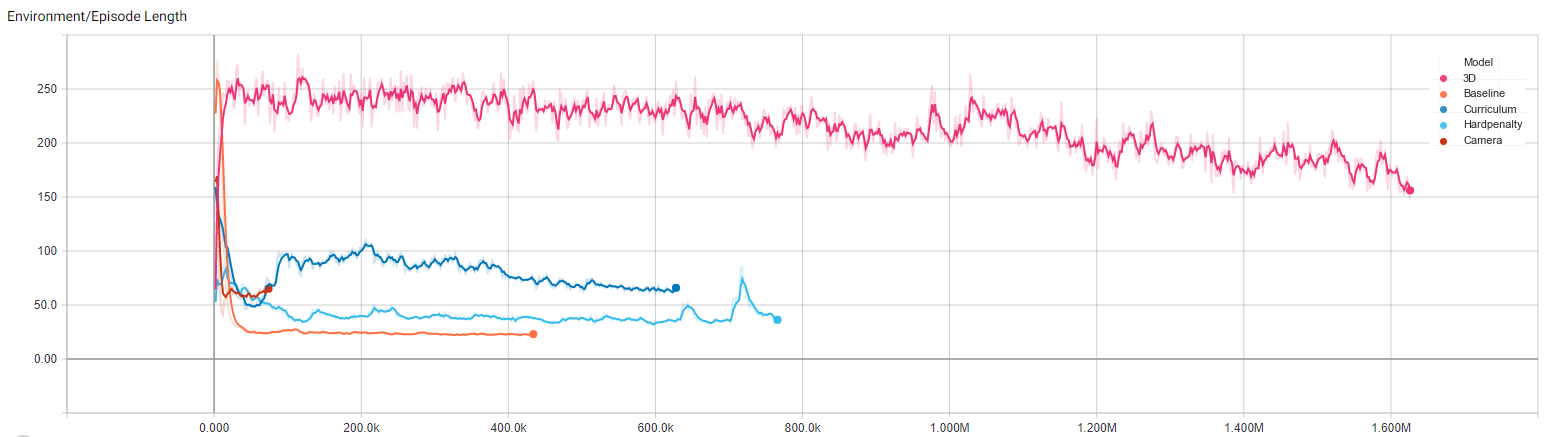
\includegraphics[width=\linewidth]{res/episode_length.PNG} 
\caption{Episode length} 
\label{fig:eplen}
\end{center}
\end{figure*}

\begin{figure*}[!htb]
\begin{center}
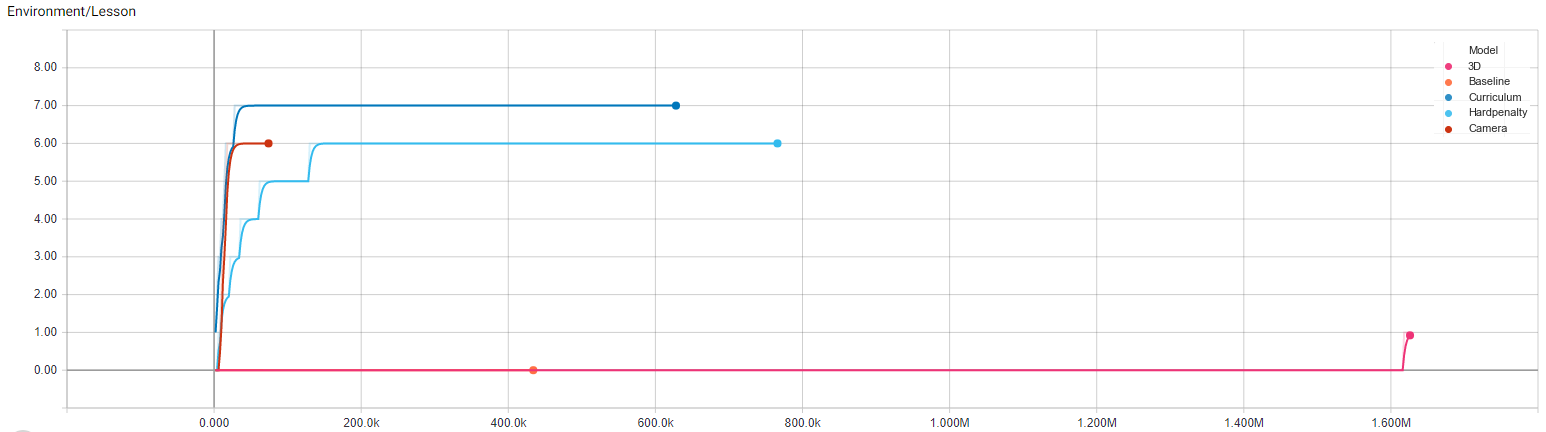
\includegraphics[width=\linewidth]{res/lesson_length.PNG} 
\caption{Curriculum lesson length} 
\label{fig:leslen}
\end{center}
\end{figure*}

\begin{figure*}[!htb]
\begin{center}
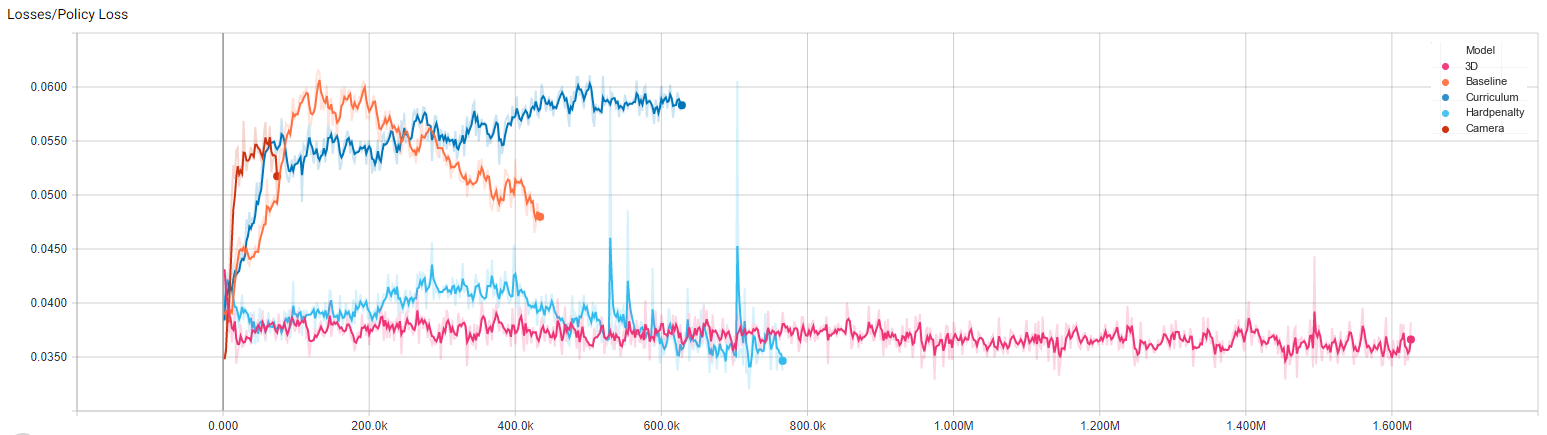
\includegraphics[width=\linewidth]{res/policy_loss.PNG} 
\caption{Policy loss (smoothed)} 
\label{fig:polloss}
\end{center}
\end{figure*}

\begin{figure*}[!htb]
\begin{center}
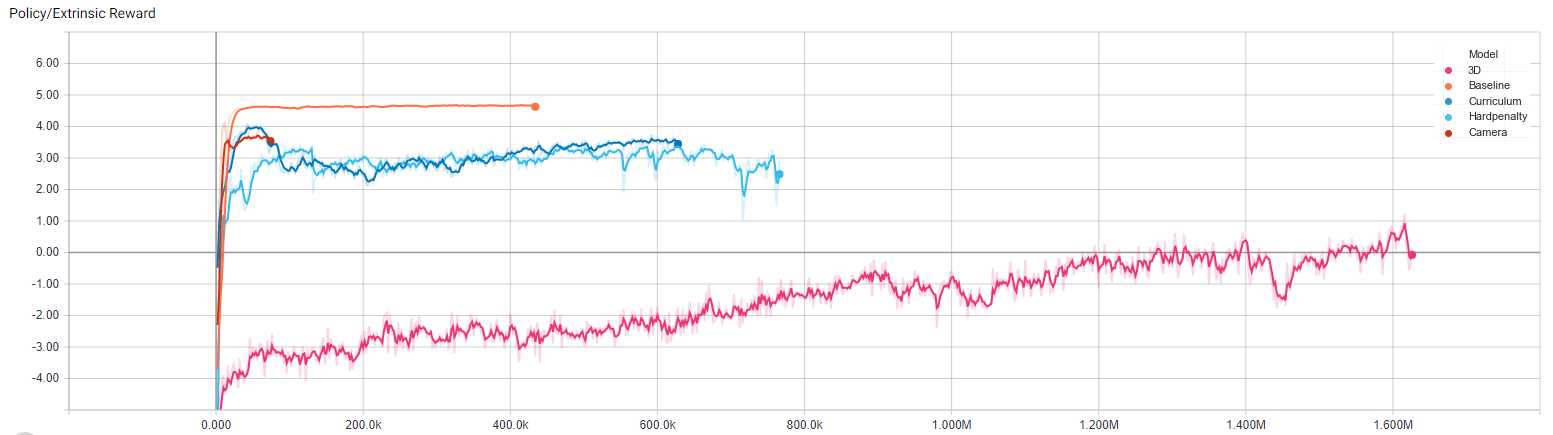
\includegraphics[width=\linewidth]{res/extrinsic_reward.PNG} 
\caption{Extrinsic reward} 
\label{fig:exrew}
\end{center}
\end{figure*}

\begin{figure*}[!htb]
\begin{center}
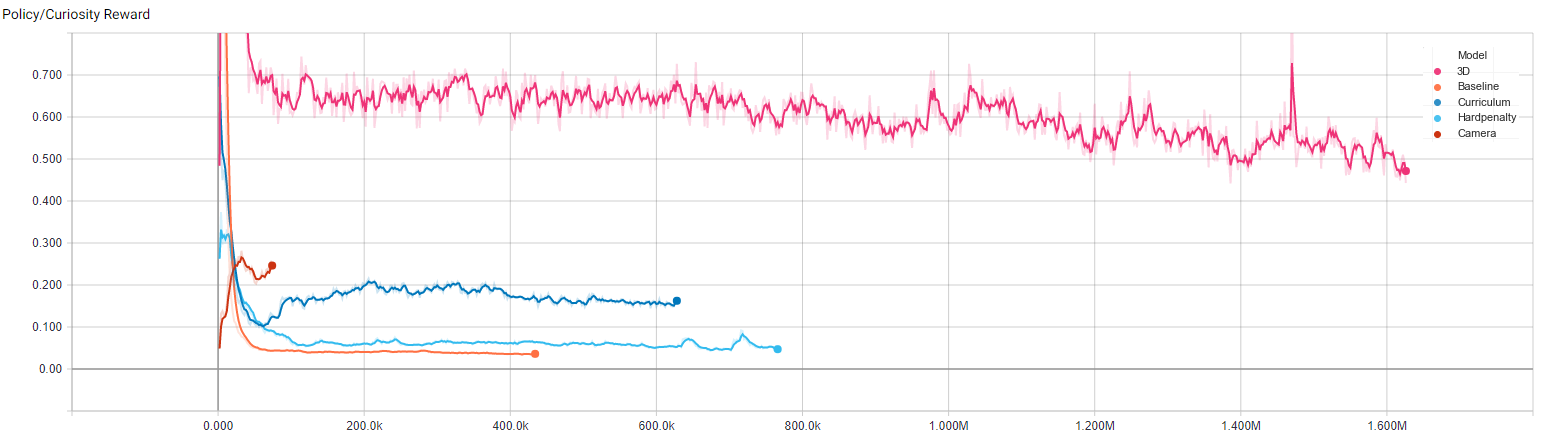
\includegraphics[width=\linewidth]{res/curiosity_reward.PNG} 
\caption{Curiosity reward} 
\label{fig:currew}
\end{center}
\end{figure*}

\section{Results and conclusions}

The empirical results show a certain decoupling between the environmental measures and the classical performance measures. Measuring performance in reinforcement learning settings is well-known to be tricky, as not always cumulative rewards, policy losses and other low-level measures are able to capture the effectiveness of the behaviour of the agent in the setting.

In the proposed setting, the experiments showed how curriculum learning can be an effective solution for improving the generalizing capabilities of the model, improving significantly how the agent behaves.

The learning system proposed shows that the policy that most commonly is converged to is a random search strategy: the agent randomly search for the environment to find the target. This is demonstrated by the behaviours of the different models - to different levels of performances - which shows the agent randomly moving between obstacles, revisiting previously seen areas until he manages to get the target in the range of its sensors. This is probably due to the randomic nature of the environment generation, as no two episodes present the same environment, and as such the agent isn't able to memorize the layout of the environment, but is only able to generally try to avoid obstacles until the targets comes into sight. 

Possible future developments are:
\begin{enumerate}
    \item \textbf{Implement memory}: adding memory to the agent (in the form of a RNN module) might allow it to form a sort of experience buffer for the current episode and allows it to explore the environment in a non-random fashion.
    \item \textbf{Rework the reward and penalty functions}: the proposed reward and penalty are pretty simplistic, a possible enhancement to the penalty could be implementing soft-collisions, that is, scaling the negative reward obtained by the agent in a collision according to the velocity of the collision - safe, soft touches can be allowed.
    \item \textbf{Compare different RL algorithms}: different reinforcement learning algorithms (A3C, DQN) might show different insights on the optimal way to implement intelligent agents in the proposed setting.
\end{enumerate}


\bibliography{bibliography}
                                          % in the appendices.
\end{document}


